\documentclass{report}
\usepackage{graphicx}
\usepackage{hyperref}
\usepackage{pdfpages}
\title{EDABA Task 1, 2, 3, 4 Report}
\author{Maciej Domański, Krzysztof Rudnicki}
\begin{document}
\maketitle
\chapter{Task 1 - Textual description of a database}
\section{Aim}

Football manager database in order to be able to simulate football manager game. \\ 
It needs to reflect realistically status, description, attributes of entities connected with football in order to ensure better simulation. \\ 


\section{Objects}  \label{Objects Section}
We have chosen to make 6 entities \\ 
\begin{itemize}
    \item Player - Football players are the most important part of this database, they take part in matches on behalf of the club, and their skill is main determinant of the outcome of games.
    \item Club - Represents football club - entity build around the football team which incorporates staff, players. Football teams represent clubs in competitions and club handles their wages. 
    \item Match - Game governed within football regulations between two football teams.
    \item Manager - Responsible for managing team, picking squad, organizing training, buying players, handling team conflicts, choosing and improving tactics. 
    \item Competition - Event where football teams play against each other in one or more matches in order to win prize. 
    \item Stadium - Venue assigned to a club where matches and competitions consisting of those matches take place.
\end{itemize} 

\section{Requirements concerning data}
Players and Manager skill is between 1 and 10 \\ 
Positions are restricted to Goalkeeper, Defender, Midfield and Attacker \\ 
Reputations ( for player, manager, club and match) are restricted between 1 and 5 (as in stars with 1 between each step) \\
Quality of facilities are restricted between 1 and 5 \\ 
Competition should have at least one match \\ 
Weather restricted to Sunny, Rainy, Snowy, \\ 
Contract can be active or expired \\

\section{Business Activities}
Activities we would like to cover are, players exchanged between clubs, player signed to club, player released from club (end of contract for example)
\\
clubs taking part in matches, clubs hiring players and manager, clubs taking part in competition, 
players playing in matches \\
manager exchanged between clubs, manager signed to club, manager released from club, \\ 
Competition organizing matches \\
Stadium ticket price being raised by club \\
Get Competition schedule from list of matches 

\chapter{Task 2 - ERD - Entity Relationship Diagram}
\begin{figure}[htpb]
    \centering
    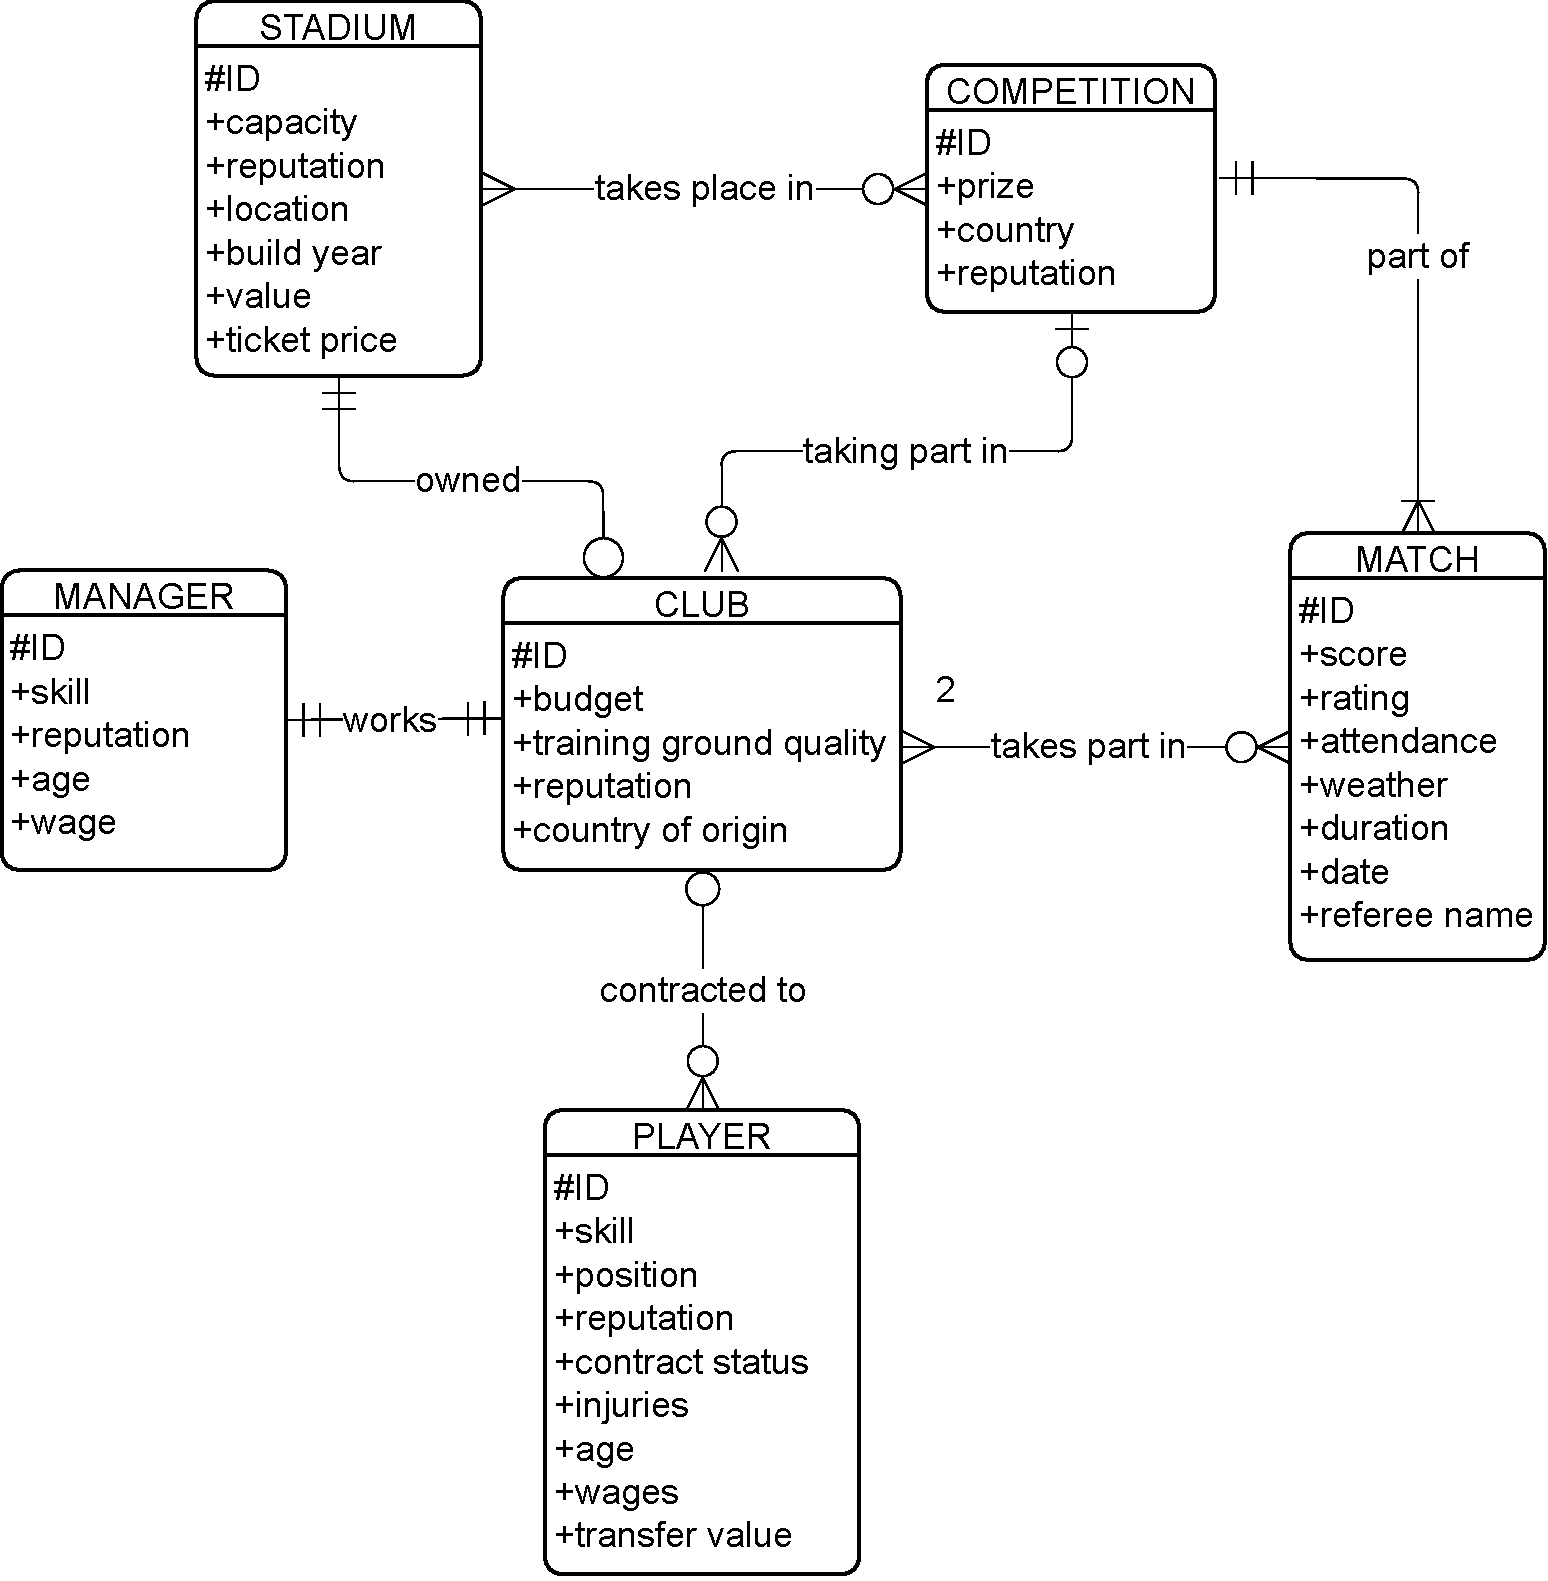
\includegraphics[width=0.8\textwidth]{erd.pdf}
    \caption{ERD}
    \label{fig:tikzpgf}
\end{figure}

\section{Description}
\subsection{Relationship description}

\paragraph{Stadium      $\rightarrow$ Competion}
Stadium can belong to many Competitions.

\paragraph{Competion    $\rightarrow$ Stadium}
Competitions take part in specific Stadiums.

\paragraph{Competion    $\rightarrow$ Match}
Competition is composed of many Matches.

\paragraph{Match        $\rightarrow$ Competion}
Match takes part within specific Competition.

\paragraph{Competion $\rightarrow$ Club}
Competition consists of many clubs.

\paragraph{Club $\rightarrow$ Competion}
Club takes part if one or none Competition at a time.

\paragraph{Club $\rightarrow$ Stadium}
Club has Stadium.

\paragraph{Stadium $\rightarrow$ Club}
Stadium may belong to a Club.

\paragraph{Manager $\rightarrow$ Club}
Manager works in one Club.

\paragraph{Club $\rightarrow$ Manager}
Club employs one Manager.

\paragraph{Club $\rightarrow$ Player}
Club may employ many Players.

\paragraph{Player $\rightarrow$ Club}
Player may be contracted to a (one) Club.

\paragraph{Match $\rightarrow$ Club}
Match is played between two Clubs.

\paragraph{Club $\rightarrow$ Match}
Club may take part in many Matches.


\subsection{Entities and attributes description}
\paragraph{Stadium}
Stadium entity represents Stadium object from \hyperref[Objects Section]{Objects Section}
\begin{itemize}
    \item capacity - maximum number of fans that can attend Match
    \item reputation - how popular it is
    \item location - where is it located
    \item build year - when it was build
    \item value - how much is it worth
    \item ticket price - price to enter a Stadium per person
\end{itemize}


\paragraph{Competition}
Competition entity represents Competition object from \hyperref[Objects Section]{Objects Section}
\begin{itemize}
    \item prize - Sum of money received by winning Club
    \item country - Where the Competition is taking place
    \item reputation - how popular it is
\end{itemize}


\paragraph{Manager}
Manager entity represents Manager object from \hyperref[Objects Section]{Objects Section}
\begin{itemize}
    \item skill - how good the Manager is at managing Club
    \item reputation - how popular Manager is
    \item age - how old the Manager is
    \item wage - how much is the Manager paid monthly
\end{itemize}


\paragraph{Club}
Club entity represents Club object from \hyperref[Objects Section]{Objects Section}
\begin{itemize}
    \item budget - amount of money it can spend yearly
    \item training ground quality - how good training grounds are
    \item reputation - how popular it is
    \item country of origin - where it was created
\end{itemize}


\paragraph{Match}
Match entity represents Match object from \hyperref[Objects Section]{Objects Section}
\begin{itemize}
    \item score - current Match score
    \item rating - how enjoyable was the game
    \item attendance - how many people came
    \item weather - weather condition during the match
    \item duration - duration of the game
    \item date - when the game took place
    \item referee name - who refereed the game
\end{itemize}


\paragraph{Player}
Player entity represents Player object from \hyperref[Objects Section]{Objects Section}
\begin{itemize}
    \item skill - how good the Player is
    \item position - position the Player is the best at
    \item reputation - how popular Player is
    \item contract status - whether the Player has active contract with a Club or is it expired
    \item injuries - days until healed (0 if no injuries present)
    \item age - how old the Player is
    \item wages - how much the Player is paid monthly
    \item transfer value - how much the Player is worth
\end{itemize}

\chapter{Task 3 - Relational schema}
\section{Relational schema}
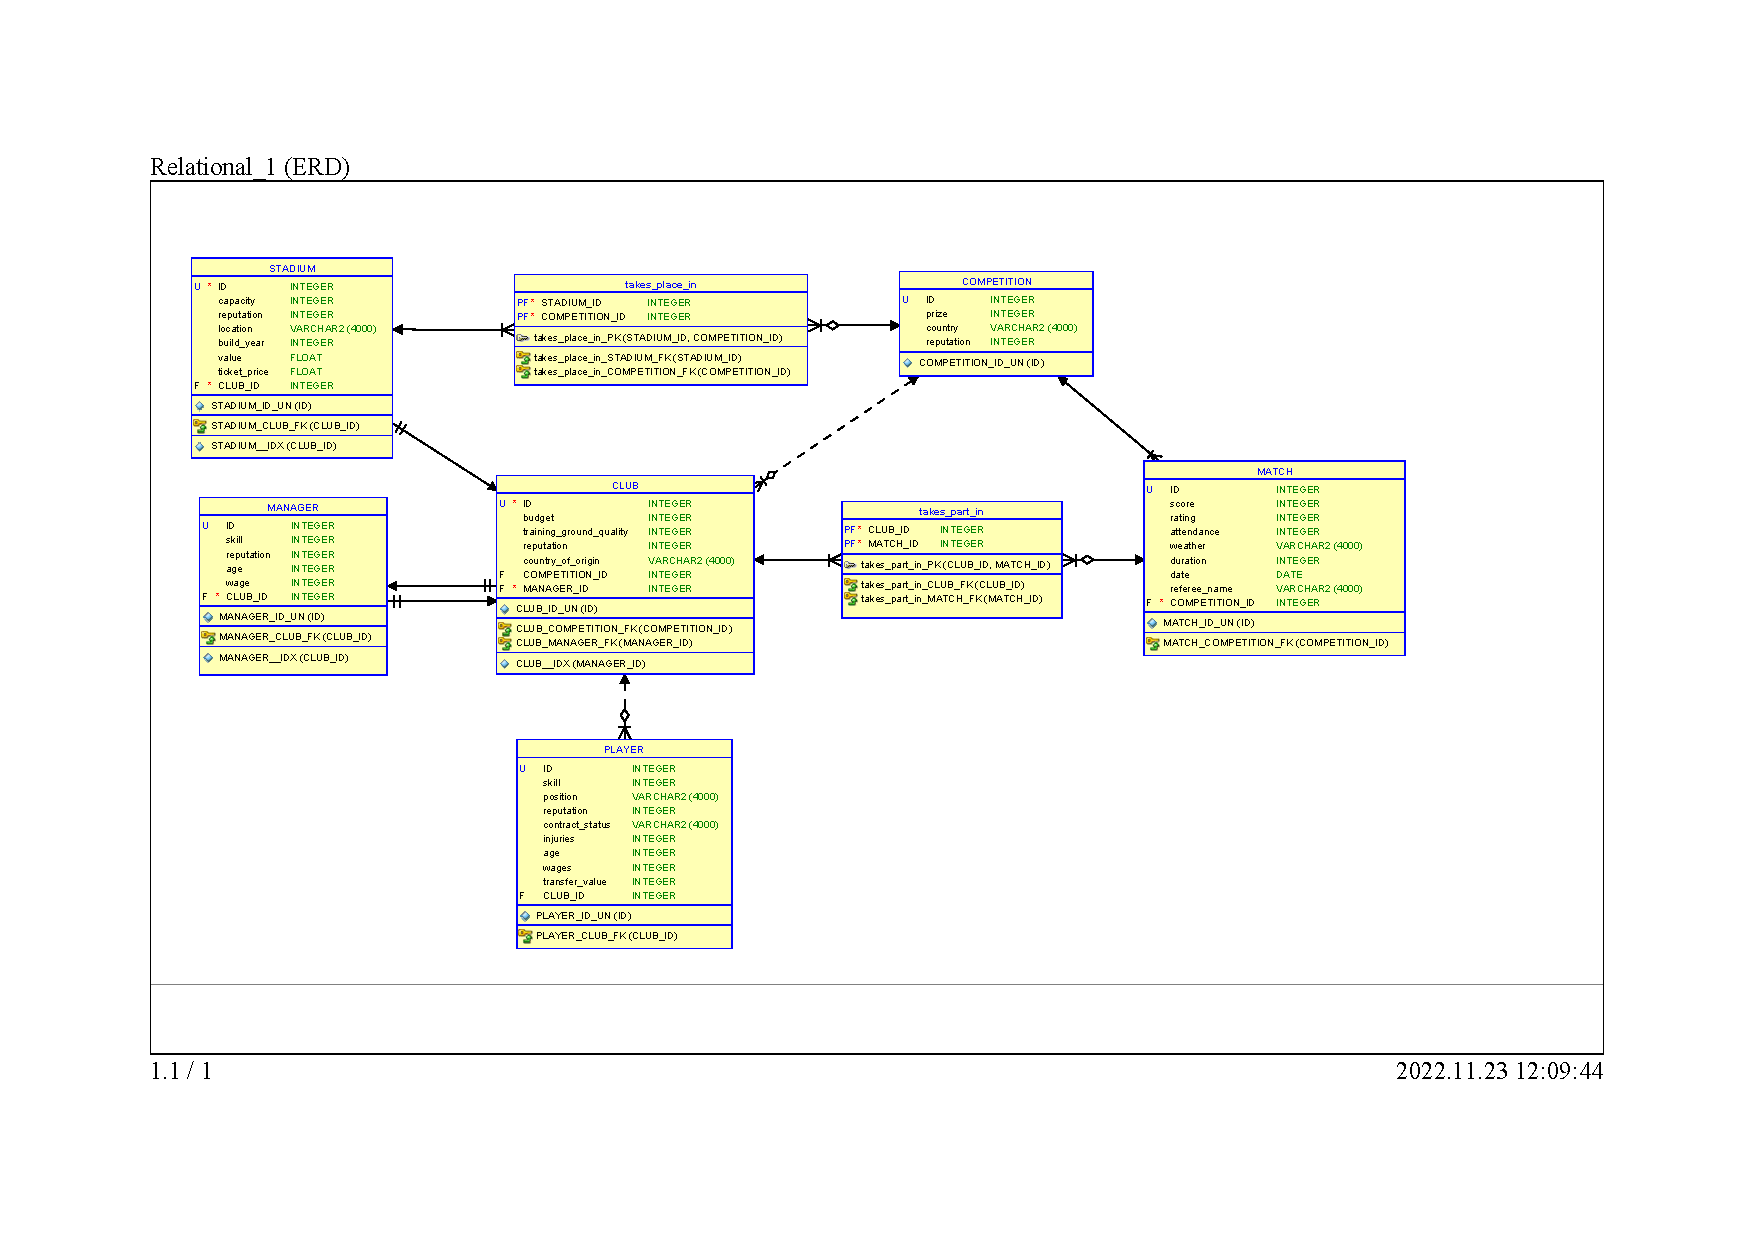
\includepdf[pages=1]{relational.pdf}
\section{Description}
A relational diagram was generated using SQL developer. The most notable aspects of it are:\\
\\
\paragraph{Entities descriptions}
How entities changed, from logical diagram:\\
In every entity we now have foreign keys to entities with whom entity has relations. In case of many to many relations new data blocks containing information about keys of two connected entities were created 
\paragraph{Relations descriptions}
How relations changed from logical diagram. \\ 
Most of the relations remained visually the same aside from three, those are:
\begin{itemize}
\item STADIUM:COMPETITION-takes\_place\_in along with CLUB:MATCH-takes\_part\_in have been separated into a relational block based on the fact that those are N:M relations
\item MANAGER:CLUB-works was disjoined into two relations due to the original relation being 1:1 with identity
\end{itemize}


\end{document}